%-------------------------------
% use environment settings for Def file, bib files, postscripts
% setenv TEXPICTS  ${HOME}/Latex/Inputs:
% setenv TEXINPUTS ${HOME}/Latex/Inputs:${HOME}/Latex/Tuletter:${HOME}/Latex/Def:
% setenv BIBINPUTS ${HOME}/Latex/Bib:

%\documentclass[11pt,twoside,fleqn]{thesis}
\documentclass[11pt,twoside,fleqn]{report}
\pagestyle{headings}

%\usepackage[scaled=0.92]{helvetrm}
\usepackage[scaled]{helvet}
\renewcommand\familydefault{\sfdefault} %% Only if the base font of
                                        %% the document is to be sans serif
\usepackage{listings}
% \usepackage{natbib}

% \usepackage{chapterbib}
\usepackage{amsmath}
\usepackage{amssymb}
\usepackage{graphics}
\usepackage{tabularx}
\usepackage{booktabs} 
\usepackage{lscape}
\usepackage{rotating}
\usepackage[dvips]{epsfig}

\usepackage{psfrag}
\usepackage[english]{babel}

\usepackage{graphicx} 
\usepackage{graphics}
\usepackage[dvips]{epsfig}
%\usepackage{longtable}
\usepackage{latexsym}
%\usepackage{xspace}
\usepackage{psfrag}
%\usepackage{fancyvrb} % fancy verbatim with fontsize, color, etc. VerbatimInput for FAQ
%\usepackage{color}
\bibliographystyle{agu}
\usepackage{natbib}
\usepackage[dvips, bookmarks, colorlinks=false, linkcolor=blue, urlbordercolor={0 0 1},citebordercolor={1 0 0},pdftitle={StaMPS/MTI Manual}, pdfauthor={Andy Hooper }, pdfkeywords={PS, PSI, MT-InSAR, StaMPS}]{hyperref}
%\usepackage{url}
\usepackage[usenames]{color}
\newcommand{\cs}[1]{{\texttt{\color{RoyalBlue}#1}}}
\newcommand{\cc}[1]{{\texttt{\color{Red}#1}}}
\usepackage[left=3cm,top=3cm,bottom=2cm,right=2.5cm]{geometry}
\emergencystretch=100pt



%\newcommand{\boxxed}[1]{\fbox{$\displaystyle{#1}$}}

\newcommand\ul{\underline}
\newcommand\ol{\overline}
\newcommand\bl{\begin{lstlisting}}
\newcommand\el{\end{lstlisting}}


\newcommand{\SWVER}{v3.2}% 

% COMMAND ABBREVIATIONS
\newcommand{\be}{\begin{equation}}
\newcommand{\ee}{\end{equation}}
\newcommand{\bea}{\begin{eqnarray}}
\newcommand{\eea}{\end{eqnarray}}
\newcommand{\bi}{\begin{itemize}}
\newcommand{\ei}{\end{itemize}}
\newcommand{\bnum}{\begin{enumerate}}
\newcommand{\enum}{\end{enumerate}}
\newcommand{\benum}{\begin{enumerate}}
\newcommand{\eenum}{\end{enumerate}}

%\newcommand{\startpreface}{\pagenumbering{roman}\setcounter{page}{1}}
%\newcommand{\starttext}{\pagenumbering{arabic}\setcounter{chapter}{0}}
%\newcommand{\startappendix}{\renewcommand{\chaptername}{Annex}\renewcommand{\thechapter}{\Alph{chapter}}\setcounter{chapter}{0}}
%
% CONSISTENCY
\newcommand{\pipe}{\ensuremath{\:|\:}}
\newcommand{\half}{\ensuremath{{1\over2}}}
\newcommand{\degs}{\ensuremath{^\circ}}
%
% TYPOS
\newcommand{\phie}{\ensuremath{\phi}}
\newcommand{\fie}{\ensuremath{\phi}}
\newcommand{\alfa}{\ensuremath{\alpha}}
%
% UNDERLINE
\newcommand{\alphau}{\ensuremath{\underline{\alpha}}}
\newcommand{\alfau}{\ensuremath{\underline{\alpha}}}
\newcommand{\betau}{\ensuremath{\underline{\beta}}}
\newcommand{\gammau}{\ensuremath{\underline{\gamma}}}
\newcommand{\xu}{\ensuremath{\underline{x}}}
\newcommand{\yu}{\ensuremath{\underline{y}}}
\newcommand{\zu}{\ensuremath{\underline{z}}}
%
% OVERLINE
\newcommand{\alphao}{\ensuremath{\overline{\alpha}}}
\newcommand{\alfao}{\ensuremath{\overline{\alpha}}}
\newcommand{\betao}{\ensuremath{\overline{\beta}}}
\newcommand{\gammao}{\ensuremath{\overline{\gamma}}}
\newcommand{\xo}{\ensuremath{\overline{x}}}
\newcommand{\yo}{\ensuremath{\overline{y}}}
\newcommand{\zo}{\ensuremath{\overline{z}}}
%
% DOT
\newcommand{\alphad}{\ensuremath{\dot{\alpha}}}
\newcommand{\alfad}{\ensuremath{\dot{\alpha}}}
\newcommand{\betad}{\ensuremath{\dot{\beta}}}
\newcommand{\gammad}{\ensuremath{\dot{\gamma}}}
\newcommand{\xd}{\ensuremath{\dot{x}}}
\newcommand{\yd}{\ensuremath{\dot{y}}}
\newcommand{\zd}{\ensuremath{\dot{z}}}
%
% DUBBLE DOT
\newcommand{\alphadd}{\ensuremath{\ddot{\alpha}}}
\newcommand{\alfadd}{\ensuremath{\ddot{\alpha}}}
\newcommand{\betadd}{\ensuremath{\ddot{\beta}}}
\newcommand{\xdd}{\ensuremath{\ddot{x}}}
\newcommand{\ydd}{\ensuremath{\ddot{y}}}
\newcommand{\zdd}{\ensuremath{\ddot{z}}}
%
% VECTOR
\newcommand{\alphav}{\ensuremath{\vec{\alpha}}}
\newcommand{\alfav}{\ensuremath{\vec{\alpha}}}
\newcommand{\betav}{\ensuremath{\vec{\beta}}}
\newcommand{\gammav}{\ensuremath{\vec{\gamma}}}
\newcommand{\xv}{\ensuremath{\vec{x}}}
\newcommand{\yv}{\ensuremath{\vec{y}}}
\newcommand{\zv}{\ensuremath{\vec{z}}}
%
% HAT
\newcommand{\alphah}{\ensuremath{\hat{\alpha}}}
\newcommand{\alfah}{\ensuremath{\hat{\alpha}}}
\newcommand{\betah}{\ensuremath{\hat{\beta}}}
\newcommand{\gammah}{\ensuremath{\hat{\gamma}}}
\newcommand{\xh}{\ensuremath{\hat{x}}}
\newcommand{\yh}{\ensuremath{\hat{y}}}
\newcommand{\zh}{\ensuremath{\hat{z}}}
%
% SINE
\newcommand{\sina}{\ensuremath{\sin{\alpha}}}
\newcommand{\sinb}{\ensuremath{\sin{\beta}}}
\newcommand{\sinc}{\ensuremath{\sin{\gamma}}}
\newcommand{\sint}{\ensuremath{\sin{\theta}}}
%
% COSINE
\newcommand{\cosa}{\ensuremath{\cos{\alpha}}}
\newcommand{\cosb}{\ensuremath{\cos{\beta}}}
\newcommand{\cosc}{\ensuremath{\cos{\gamma}}}
\newcommand{\cost}{\ensuremath{\cos{\theta}}}
%
% FOURIER
%\newcommand{\FTsymbol}{\matcal{F}}
\newcommand{\FTsymbol}{\it {FT}}
\newcommand{\IFTsymbol}{\matcal{F^{-1}}}
\newcommand{\FT}{\stackrel{\FTsymbol}{\longleftrightarrow}}
%
% Consistency in used words
\newcommand{\resfile}{{\bf result file}\xspace}
\newcommand{\resfiles}{{\bf result files}\xspace}
\newcommand{\mresfile}{{\bf master result file}\xspace}
\newcommand{\sresfile}{{\bf slave result file}\xspace}
\newcommand{\iresfile}{{\bf products result file}\xspace}
\newcommand{\inputfile}{{\bf input file}\xspace}
\newcommand{\inputfiles}{{\bf input files}\xspace}
\newcommand{\outputfile}{{\bf output file}\xspace}
\newcommand{\outputfiles}{{\bf output files}\xspace}
\newcommand{\makefile}{Makefile\xspace}
\newcommand{\pcf}{{\bf process control flag}\xspace}
\newcommand{\pcfs}{{\bf process control flags}\xspace}

%%% newcommands
\newcommand{\Bpar}{{B_{\parallel}}}
\newcommand{\Bperp}{{B_{\perp}}}
\newcommand{\Bh}{{B_{h}}}
\newcommand{\Bv}{{B_{v}}}
\newcommand{\KK}{\frac{4\pi}{\lambda}}
\newcommand{\Bperpref}{{B_{{\perp0}}}}
\newcommand{\Bparref}{{B_{{\parallel0}}}}

% too unclear: \newcommand{\pi4lam}{\ensuremath{-{4\pi\over\lambda}}}
%%% style for mandatory/optional Keywords
\newlength{\MY}
\setlength{\MY}{\linewidth}
%\addtolength{\MY}{30em}%			indent parbox
\addtolength{\MY}{2em}%			indent parbox
% \addtolength{\MY}{\linewidth}%			indent parbox
\newcommand{\man}[3]{
  {\textsf{\bf{#1}}}
    \hfill\parbox[t]{.75\linewidth}{
  {\textrm{\it{#2}}}}\\
    \phantom{mm}\parbox[t]{\MY}
  {#3}\\[3ex]}%	indent parbox
\newcommand{\opt}[3]{
  {\textsf{   {#1}}}
    \hfill\parbox[t]{0.75\linewidth}{
  {\textrm{\it{#2}}}}\\
    \phantom{mm}\parbox[t]{\MY}
  {#3}\\[3ex]}%	indent parbox
%%% style for optional/default parameters

\newcommand{\defpm}[1]{{\underline{#1}}}
\newcommand{\optpm}[1]{\textnormal{[} {#1} \textnormal{]}}

% These three commands make up the entire times.sty package.
\renewcommand{\sfdefault}{phv}
\renewcommand{\rmdefault}{ptm}
\renewcommand{\ttdefault}{pcr}
% enable Times now - so that all class options can see the correct font families
\normalfont\selectfont

%============================================
\begin{document}
\setlength{\parskip}{8pt}

%\lstlistoflistings
\definecolor{listinggray}{gray}{0.90}
\definecolor{notegray}{gray}{0.75}

\lstset{language=c++,                % choose the language of the code
  basicstyle=\small\ttfamily,    % the size of the fonts that are used for the code
  commentstyle=\small\ttfamily,
  showstringspaces=false,             % underline spaces within strings
  numbers=left,                       % where to put the line-numbers
  numberstyle=\footnotesize\sffamily, % the size of the fonts that are used for the line-numbers
  firstnumber=0,
  stepnumber=0,                       % the step between two line-numbers. If it's 1 each line will be numbered
  numbersep=10pt,                     % how far the line-numbers are from the code
  numberblanklines=false,
  backgroundcolor=\color{listinggray},% choose the background color. You must add \usepackage{color}
  showspaces=false,                   % show spaces within strings adding particular underscores
  showtabs=false,                     % show tabs within strings adding particular underscores
  % frame=single,                     % adds a frame around the code
  tabsize=2,                          % sets default tabsize to 2 spaces
  captionpos=b,                       % sets the caption-position to bottom
  breaklines=true,                   % sets automatic line breaking
  breakatwhitespace=false,            % sets if automatic breaks should only happen at whitespace
  escapeinside={\%*}{*)}              % if you want to add a comment within your code
}


\thispagestyle{empty}
  
\begin{center}
{\sffamily\Huge{\textbf{\textsc{\\}}}}
  \vspace{0cm}
  {\sffamily\Huge{\textbf{{\\
   StaMPS/MTI  Manual\\
     }}}}
     \vspace{5mm}
     {\sffamily\Large{\textbf{Version 3.2}}}
\vspace{5mm}


\end{center}

\begin{center}
  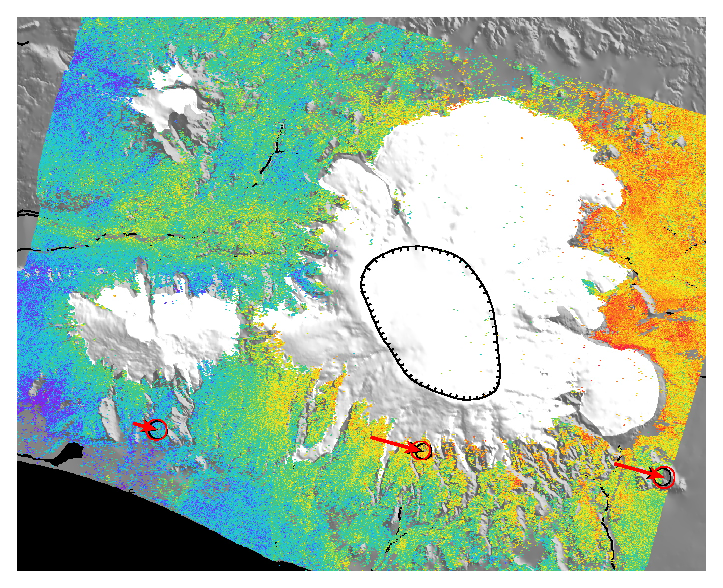
\includegraphics[width=0.85\linewidth]{./figs/title3}
\end{center}
\vspace{0mm}

%\begin{flushright}
\begin{center}
{\sffamily\textbf{Andy Hooper, Karsten Spaans, David Bekaert, Miguel Caro Cuenca, Mahmut Ar{\i}kan.\\
4th November, 2010}}
%\end{flushright}
\end{center}


\vspace{20mm}


    %\begin{minipage}[b]{1.0\linewidth}      
      \begin{minipage}[b]{0.3\linewidth}
        
\includegraphics[width=\linewidth]{./figs/TUDelft_logo}
      \end{minipage}\hfill
      \begin{minipage}[b]{0.67\linewidth}
        \begin{flushright}
          {\sffamily
          \textbf{Delft Institute of Earth Observation and Space Systems}\\\textbf{Delft University of Technology}\\
          Kluyverweg 1, 2629 HS, Delft\\
          The Netherlands}
        \end{flushright}
      \end{minipage}

    %\end{minipage}

\vspace{0mm}
\newpage
\pagenumbering{roman}
\setcounter{page}{1}
%\include{preface}
\setlength{\parskip}{0pt}
\tableofcontents
\setlength{\parskip}{8pt}

%
\newpage
\pagenumbering{arabic}


%KNIP

%\setlength{\parskip}{4pt}
%\pagenumbering{\sffamily roman}
%\maketitle
%\addcontentsline{toc}{chapter}{Summary}
%\addcontentsline{toc}{chapter}{Nomenclature}
%{\sffamily \tableofcontents}


\setlength{\unitlength}{1mm}
\setlength{\parindent}{0.0cm}
\setlength{\parskip}{10pt}








\chapter{Introduction}

StaMPS/MTI is made available for non-commercial applications only. 

StaMPS (Stanford Method for Persistent Scatterers)  is a software package that implements an InSAR persistent scatterer (PS) method developed to work even in terrains devoid of man-made structures and/or undergoing non-steady deformation. StaMPS/MTI (Multi-Temporal InSAR) is an extended version of StaMPS that also includes a small baseline method and a combined multi-temporal InSAR method. The original development of StaMPS was undertaken at Stanford University, but subsequent development of StaMPS and StaMPS/MTI has taken place at the University of Iceland and Delft University of Technology. There are also contributions from users of the package based at other institutions.

This manual provides a guide to running StaMPS/MTI, but does not  explain all the processing. For some details on the inner workings, see \citet{HooperA2010b,HooperA2008,HooperA2007a,HooperA2004,HooperA2006}.
 %Hooper and Zebker (2007) and Hooper, Ph.D Thesis. 
 
 A user group is also maintained at \url{http://groups.google.com/group/mainsar}. If you have a query, check the discussion threads there and, if not resolved, submit your question to the group.




There are two pre-processing steps before getting to the PS/MTI processing proper. The first is to focus the raw data (if required), and the second is to form interferograms from single-look complex (SLC) images. ROI\_PAC is used for the focusing and Doris for interferogram formation. If starting with CEOS format SLC images, rather than raw data, the focusing step is skipped and the images are imported directly into Doris. Currently, support is provided for processing ERS, Envisat or ALOS data, if starting with raw data, and for  ERS, Envisat or RADARSAT-1 data, if starting with CEOS SLCs.





 Both  ROI\_PAC and Doris processing are non-standard and various shell scripts, matlab scripts and programs are included in this package to produce interferograms that are PS/MTI friendly.





 The PS/MTI processing itself includes C++ programs and matlab scripts  to identify coherent pixels, and to extract the deformation signal for these pixels. Typing \cs{help} followed by the name of the matlab script  provides a brief description of the processing.





 Throughout this manual, commands to be entered on the command line are in \cs{blue}
and entries that are specific to the data set being processed and require modification are in \cc{red}. The presence of $>>$ before a command indicates that the command is a matlab script.



\chapter{Installation}


%StaMPS is designed to run under the tcsh shell (you can usually invoke this by typing \cs{tcsh} from whatever shell you are within). Alternatively adapt {\tt StaMPS\_CONFIG} for your favourite shell.


 Install StaMPS/MTI: \\
 \cs{ tar -xvf StaMPS\_v3.2.tar\\
 cd StaMPS\_v3.2/src\\
 make\\
 make install}

\section{Configuration}
Edit {\tt StaMPS\_CONFIG.tcsh} or {\tt StaMPS\_CONFIG.bash} (depending on which shell you prefer to use) to point to the correct directories for your set-up (you will need additional programs installed, see below).\\
 \cs{source StaMPS\_CONFIG.}\cc{xxxx}
 \\
  This must be done whenever a new terminal is opened. You might want to add this line to your {\tt.cshrc} or {\tt.bashrc} file so that this is done automatically.

\section{Data display}
A program called dismph (to display complex data)  is included in the package but not compiled by default. It uses X11 Open Motif. This is installed as standard under many unix/linux operating systems, and can be installed on OS X systems from:  \url{http://fink.sourceforge.net/}.
 Copy {\tt include/Xm} to {\tt /usr/X11R6/include} and {\tt libXm.a} to {\tt /usr/X11R6/lib}.
 To compile dismph, run\\
 \cs{make dismph}.
 
 Alternatively another display program may be used instead of dismph, e.g.,\\ xv (\url{http://www.trilon.com/xv}) or OpenEV (\url{http://fwtools.maptools.org/}).


\section{ROI\_PAC}
Details on installing and running ROI\_PAC (if needed) can be found at:
\\ \url{http://roipac.org/ROI_PAC}.

For ERS, ROI\_PAC requires the program getorb which must be installed in the {\tt ROI\_PAC/INT\_BIN} directory and can be downloaded from:\\ 
\url{http://www.deos.tudelft.nl/ers/precorbs/tools/getorb_pack.shtml}.

ODR and arclist files containing the orbit information used by getorb can be downloaded from:\\ 
\url{http://www.deos.tudelft.nl/ers/precorbs/orbits/}.\\
These files should be stored in directories {\tt .../ODR/}\cc{XXXX} where \cc{XXXX} is {\tt ERS1} or {\tt ERS2}.   For Envisat data, getorb can also be used, in which case \cc{XXXX} should be {\tt Envisat}. Alternatively, use the ESA DORIS (the tracking system on Envisat, not to be confused with the Doris interferometry software) orbits. This is a better option at the date of writing as the ODR files have not been updated since the beginning of 2008.



\section{Doris}
 Details on installing Doris can be found at:\\
  \url{http://doris.tudelft.nl} .



\section{Triangle}
 The Triangle program is used for Delaunay triangulation and can be found at:\\
  \url{http://www.cs.cmu.edu/~quake/triangle.html}.
 
 \section{Snaphu}
 The optimisation routines of snaphu are used by the 3-D unwrapping code and can be downloaded from:\\
  \url{http://www-star.stanford.edu/sar_group/snaphu}.






 
\chapter{Create SLCs (using ROI\_PAC)}

Currently support is provided for raw data from ERS, Envisat and ALOS satellites.



{\em If you are starting with SLC data rather than raw data, skip this section.}




 Scripts have been updated to run with ROI\_PAC version 2.3 or 3.0. If you have the ROI\_PAC version 2.2 installed, you should run the versions of the SLC generation scripts with the suffix \cs{\_V2.2} attached.



 In your processing directory:\\
 \cs{mkdir SLC}\\
 \cs{cd SLC}\\
 %\cs{cp \$MY\_SCR/roi.proc .}\\
 \cs{mkdir} \cc{yyyymmdd}
 for each scene and within this directory create symbolic links to the raw data (and leader files if they exist). For ERS data the link names must be {\tt IMAGERY}\cc{yyymmdd} and {\tt SARLEADER}\cc{yyyymmdd} (\underline{be sure to use 4 digit, not 2 digit, years}), but for Envisat and ALOS data the link names should be the same as the original names.\\
 The script \cs{link\_raw} can be used to automatically set-up the directory structure SLC/\cc{yyyymmdd} for ERS (CEOS and Envisat format), Envisat and ALOS platforms. Type \\
\cs{link\_raw }   \cc{ data\_path }   \cc{ processing\_path}, \\
with \cc{data\_path} the path to your source data and \cc{processing\_path} the path where the processing SLC dir and symbolic links need to be created.\\
 

 Choose a master based on minimising perpendicular, Doppler and temporal baselines (see \citet{HooperA2007a}). If you do not know the baseline data, choose a preliminary master based only on time and follow this manual as far as the {\tt make\_coarse} step in Section \ref{sec:ifgs}. After running {\tt make\_coarse}, the script {\tt select\_master} can be used to calculate expected stack coherence. Alternatively, one can enter \cs{grep Bperp */coreg.out} in the {\tt INSAR\_}\cc{master\_date} directory to see the perpendicular baselines with respect to the selected master (enter \cs{grep f\_DC\_con */slave.res} in the {\tt SLC} directory for the Doppler centroids). A new master can then be picked if necessary. If this is the case, edit {\tt master\_crop.in} for the new master, run \cs{step\_master\_setup},  then go directly to Section \ref{sec:ifgs}.
 
 
 Substitute your chosen master date in the format {\tt yyyymmdd} wherever \cc{master\_date} appears below.





 From the SLC directory:


 %\cs{echo} \cc{master\_date} \cs{$>$ make\_slcs.list }\\
 %\cs{make\_slcs\_ers } or \cs{make\_slcs\_envi}\\
 \cs{cd} \cc{master\_date}
 
  
  
 To use ODR orbits:\\
 \cs{step\_slc\_ers} or \cs{step\_slc\_envi} (use \cs{\_V2.2} suffix if necessary)\\
 To use DORIS orbits (Envisat only):\\
 \cs{step\_slc\_envi\_vor}\\ 
 For ALOS data:\\
  \cs{step\_slc\_alos}\\
 %\cs{multilook} \cc{master\_date}\cs{.slc} \cc{5612 }
%(or whatever is the filewidth - check \cc{master\_date}\cs{.slc.rsc})\\
 %\cs{dismph} \cc{master\_date}\cs{.slc.4looks} \cc{1403 }
%(former filewidth/4)
For ERS in Envisat type format:\\
 \cs{step\_slc\_ers\_envi}\\
In this case you need to update ROI-PAC with the programs provided in\\
 \url{http://www.roipac.org/ERS}


Take note of the number of azimuth/range looks and the multilooked filewidth.
 
 \cs{dismph image.slc.}\cc{X}\cs{looks.raw} \cc{1294 } (range looks, multilooked filewidth) or\\
  \cs{xv image.slc.}\cc{X}\cs{looks.ras}



Choose your region of interest and note the first/last azimuth lines and first/last range pixels. You should try to pick an area that is included in all the slave images too, which may not be the case if you choose an area too close to the image edge. Multiply the line numbers by the number of azimuth looks and the pixel numbers by the number of range looks to get line/pixel numbers referenced to the SLC. 

%Choose area of interest and note first and last azimuth line numbers (multiplying by 20) e.g. 15000 and 20000 and first and last range pixel numbers (multiplying by 4) e.g. 2400 and 3400



 %\cs{cd ..} (back to SLC directory)\\
Edit {\tt../roi.proc} and change the following:\\
%\begin{list}{}{}
% {\tt before\_z\_ext = {\color{Red}-12500} -}(first az line minus 2500) N.B., include the minus sign\\
%{\tt number\_of\_patches = {\color{Red}3}} ((last line - first line + 2500)/3000 rounded up)\\
{\tt ymin = {\color{Red}14000}} (first azimuth line minus 1000)\\
{\tt ymax = {\color{Red}21000}} (last azimuth line plus 1000). You will also need to uncomment this line\\
{\tt mean\_pixel\_rng = {\color{Red}2900}} (range pixel of middle of region of interest)
%\end{list}



 %\cs{remake\_slcs}\\
 %\cs{cd} \cc{master\_date}\\
 \cs{step\_slc\_alos}, \cs{step\_slc\_ers},  \cs{step\_slc\_ers\_envi} or \cs{step\_slc\_envi} (attach \cs{\_V2.2} suffix if necessary).\\
 %\cs{multilook} \cc{master\_date}\cs{.slc} \cc{5612 }
%(or whatever is the filewidth)\\
 %\cs{dismph} \cc{master\_date}\cs{.slc.4looks} \cc{1403 }
%(former filewidth/4)
 \cs{dismph image.slc.}\cc{X}\cs{looks.raw} \cc{1294 } (range looks, multilooked filewidth) or\\
  \cs{xv image.slc.}\cc{X}\cs{looks.ras}



 Find your region of interest again and note the new first and last azimuth line numbers (multiplying by the number of azimuth looks) . 
 
 \cs{cp \$MY\_SCR/master\_crop.in .}\\
 Edit {\tt master\_crop.in}
and update the crop area: {\tt first\_l} and {\tt last\_l} are the first and last azimuth line numbers, {\tt first\_p} and {\tt last\_p} are the first and last range pixels. 
% If the last digits of {\tt last\_l} \& {\tt last\_p} are equal to the last digits of {\tt first\_l} \& {\tt first\_p} plus 9, the length/width will be  round numbers. 
 
 \cs{step\_master\_setup}\\
 \cs{cd ..} (back to SLC directory)


 %\cs{$\backslash$ls -d [1,2]* $>$ make\_slcs.list}\\
 %\cs{vi make\_slcs.list} and remove the entry for \cc{master\_date}\\
\cs{make\_slcs\_alos}, \cs{make\_slcs\_ers}, \cs{make\_slcs\_ers\_envi}, 
 \cs{make\_slcs\_envi} (attach \cs{\_V2.2} suffix if necessary), or  \cs{make\_slcs\_envi\_vor}. This will create SLCs for all directories listed in {\tt make\_slcs.list}, which by default contains all data directories except the master.



%If needed, \cs{remake\_slcs} will recreate SLCs for all entries in {\tt make\_slcs.list} without rerunning the {\tt make\_raw.pl} step of ROI\_PAC. 


 It may become apparent later that one or more scenes are offset from the master by so much that the focused image does not include the entire cropped master image. In which case copy {\tt roi.proc} from the SLC directory to the relevant \cc{yyyymmdd} directory, rename it {\tt \cc{yyyymmdd}.proc} and edit it so that the the part processed includes the cropped master image. Edit {\tt make\_slcs.list} to leave only scenes that need recreating and run \cs{make\_slcs\_}\cc{XXXX}. 


\chapter{Pre-processing SLCs (Level 1 product) }

{\em If you created SLCs with ROI\_PAC using raw data (Level 0 product), skip Sections: \ref{sec:slcread1} and \ref{sec:slcread2} .}

Currently, scripts exist for pre-processing (reading and cropping) single look complex (SLC) products from ERS, Envisat and RADARSAT-1 and TerraSAR-X satellites.

 In your processing directory, for example, under /mnt/iceland\_volcanos/:\\
 \cs{mkdir SLC}\\
 \cs{cd SLC}\\
 \cs{mkdir} \cc{yyyymmdd}
 %for each scene and make a symbolic link to the corresponding ASA\_IMP\_1P file, named image.slc 
for each scene and within this directory create symbolic links to the raw data (and leader/volume files if they exist). For ERS and RADARSAT-1 data the link names must be {\tt DAT\_01.001} and {\tt  LEA\_01.001} and {\tt VDF\_DAT.001}. For Envisat  data the link name must be {\tt image.slc}.

Choose a master based on minimising perpendicular, Doppler and temporal baselines (see \citet{HooperA2007a}). Substitute your master date in the format {\tt yyyymmdd} wherever \cc{master\_date} appears below.


 \cs{cd} \cc{master\_date}\\
 \cs{step\_read\_whole\_}\cc{XXX} (where \cc{XXX} is `\cs{ERS}', `\cs{Envisat}', `\cs{RSAT}', or `\cs{TSX}')
 
 Take note of the number of azimuth/range looks and the multilooked filewidth.
 
 \cs{dismph image.slc.}\cc{X}\cs{looks.raw} \cc{1294 } (range looks, multilooked filewidth) or \cs{xv image.slc.}\cc{X}\cs{looks.ras}
 
\section{\label{sec:slcread1} Option 1: Specify by latitude and longitude}
edit {\tt master\_crop\_geo.in} in the SLC directory, and specify your area of interest.  

\cs{cd} \cc{master\_date}\\
\cs{step\_master\_read\_geo\\
cd ..\\
make\_read\_geo}
 
\section{\label{sec:slcread2}Option 2: Specify by line/pixel number}
Choose area of interest and note first/last azimuth line and first/last range pixel. You should try to pick an area that is included in all the slave images too, which may not be the case if you choose an area too close to the image edge. Multiply the line numbers by the number of azimuth looks and the pixel numbers by the number of range looks to get numbers referenced to the SLC. 
%Generally you should be at least 1000 lines in azimuth and 40 pixels in range from the edges, but even this may not be enough. 



 \cs{cp \$MY\_SCR/master\_crop.in .}\\
 Edit {\tt master\_crop.in}
and update the crop area. {\tt first\_l} and {\tt last\_l} are the first and last azimuth line numbers, {\tt first\_p} and {\tt last\_p} are the first and last range pixels.
%If the last digits of {\tt last\_l} \& {\tt last\_p} are equal to the last digits of {\tt first\_l} \& {\tt first\_p} plus 9, the length and width will be round numbers

 \cs{step\_master\_read} 




 \cs{cd ..} (back to SLC directory)\\
 %\cs{$\backslash$ls -d [1,2]* $>$ make\_slcs.list}\\
 %!TEX encoding = UTF-8 Unicode\cs{vi make\_slcs.list} and remove the entry for \cc{master\_date}\\
 \cs{make\_read}\\
 This will read and crop SLCs from all directories listed in {\tt make\_slcs.list}, which by default contains all SLC directories except the master date.\\

% OVERSAMPLING
% Mahmut
\section{\label{sec:ovs} Oversampling SLC data (Optional)}

After focusing your RAW data or reading/cropping your SLCs, optionally, you can oversample your dataset using Doris.

In your processing directory, for example, under /mnt/iceland\_volcanos/:\\
 \cs{cd SLC}\\
 \cs{cd} \cc{master\_date}\\
 \cs{step\_master\_ovs}

 \cs{cd ..} (back to SLC directory)\\
 \cs{make\_ovs}\\
 This will oversample SLCs from all directories listed in {\tt make\_slcs.list}, which by default contains all SLC directories except the master date.\\

By default, oversampling is done with a factor of 2 in both range and azimuth directions. You can change this by copying files {\tt master\_ovs.dorisin} and {\tt ovsfiles.dorisin} to {\tt SLC} directory.\\
  cp {\tt \$DORIS\_SCR/master\_ovs.dorisin} {\tt SLC/}\\
  cp {\tt \$DORIS\_SCR/ovsfiles.dorisin} {\tt SLC/}

  and then edit the parameters listed under oversampling section on each file. Finally, re-run \cs{step\_master\_ovs} and \cs{make\_ovs} to create new oversampled dataset.

%add some tips in the future

\chapter{\label{sec:ifgs} Create IFGs (using DORIS)}


 In the same directory where SLC and INSAR\_\cc{master\_date} reside:\\
 \cs{mkdir DEM}



 Place your DEM in this directory. 





\cs{cd INSAR\_}\cc{master\_date}

 If the SLCs weren't created by ROI\_PAC create {\tt \cc{master\_date}.slc.rsc}
with the following line, substituting the correct heading (to the nearest degree is fine):\\
 {\tt HEADING \ \ \ \cc{-167}}

 \cs{step\_master\_orbit\_ODR} (only run if using precise ODR orbits)


 edit {\tt timing.dorisin} and update the following fields based on the DEM you are using:
 


{\tt SAM\_IN\_FORMAT  \cc{real4}\\
 SAM\_IN\_DEM\ \ \ \  \cc{/data/T156/DEM/dem\_data.flt}\\
 SAM\_IN\_SIZE\ \ \  \cc{4801 4801}\ \  // rows cols\\
 SAM\_IN\_DELTA\ \  \cc{0.000833333 0.000833333}\ \  // posting in degrees\\
 SAM\_IN\_UL\ \  \ \ \  \cc{13 42}\ \ // lat and lon of upper left\\
 SAM\_IN\_NODATA\   \cc{-9999}}







 \cs{step\_master\_timing} 


 This step can be run alongside \cs{make\_orbits}, \cs{make\_coarse} and \cs{make\_coreg}.
 This step was new in version 3.1, and replaces the former StaMPS codes for DEM offset correction with new code in  Doris v4.0. Offsets are calculated for 30 (by default) different windows, which are printed to the screen at the end. Check that the selected offsets are consistent with the mode values of for the windows. If not, change the number of windows in {\tt timing.dorisin} to a higher number, comment out the {\tt M\_SIMAMP} process and rerun the step. If still not successful, delete the output from the timing step in master.res in the INSAR\_\cc{master\_date} directory and \underline{ALL subdirectories}, and calculate the DEM offset manually (see Section \ref{sec:calcdem}). 


\begin{center}
\colorbox{notegray}{
\begin{minipage}{0.95\linewidth}
\begin{small}\textbf{Tip: } 
 \cs{step\_master\_timing}  calculates the master timing error, which is mostly used for geocoding. Non precise time information can make geocoding to place the pixels in an inaccurate position. The reliability of the estimated time error mostly depends on the DEM. For example, it is not advisable to run this step if the topography of an area is flat and the DEM does not contain information about building height. In this case, 
 \cs{step\_master\_timing} can be skipped and continue with the rest of the processing as normal.
\end{small}

 \vspace{0.5mm}
\end{minipage}
}
\end{center}


 %\cs{$\backslash$ls -d ../SLC/[1,2]* $>$ slcs.list}
 %(N.B. If the SLC directories are not in the same directory as INSAR\_\cc{master\_date}, the full path must be given)\\
 %\cs{vi slcs.list}
 %and remove \cc{master\_date}\\
 
 \section{Bulk Processing}
 
 In the INSAR\_\cc{master\_date} directory:
 
\cs{make\_orbits}

This creates a subdirectory for each slave image. The default is to treat all images in the SLC directory except the master as slave images. If a different set of slave images is required, create a file named {\tt slcs.list} listing the directories containing the images you wish to include, before running {\tt make\_orbits}. Precise orbits are extracted from the ODR files if they are found (ERS and Envisat only).


\cs{make\_coarse}

This creates a {\tt coreg.out} file in each slave subdirectory. The last 32 lines of each {\tt coreg.out} file is output to the terminal at the end.  Check the following values for each {\tt coreg.out} file:

{\tt Coarse\_correlation\_translation\_lines:  \cc{-76}\\
 Coarse\_correlation\_translation\_pixels: \cc{-1}}


 These values should be approximately the modal values from the data below them. If this is not the case and the values are wrong by more than a couple of pixels, you should edit the relevant {\tt coreg.out} file and correct the values. 
 
Optionally, you can also check that the master crop is included within each slave image (only the parts of the master crop that are in ALL slaves will be considered in the later times series processing). Look for the highest and lowest values of {\tt Coarse\_correlation\_translation\_lines} and 
 {\tt Coarse\_correlation\_translation\_pixels}. Add the translations to the master crop range (in {\tt master.res}) and make sure the corresponding slave crop contains the translated values (in {\tt slave.res}). If not, you should adjust either the master crop or the relevant slave crops. If you adjust the master crop, it is easiest to delete the whole {\tt INSAR\_\cs{master\_date}} directory and recreate it with \cs{step\_master\_setup} (raw data) or \cs{step\_master\_read}/\cs{step\_master\_read\_geo} (CEOS SLC data). If you adjust slave crops (by rerunning  \cs{step\_slc\_}\cc{XXX} or \cs{step\_read}), you need run \cs{step\_orbit} in the slave subdirectory only for those slaves that have been adjusted.  
  
 It may also be the case that there is a timing error in the orbit info and the approximate values in {\tt \_Start\_coarse\_orbits} are too far from the real values for coarse correlation to work. In this case, estimate the coarse offsets yourself (look at the SLCs), update them in {\tt \_Start\_coarse\_orbits} in {\tt coreg.out} and rerun just the Doris {\tt COARSECORR} step.




 \cs{make\_coreg}
 (long runtime) 

 By default all images with baseline $<$ 100 m are coregistered directly to the master and those with larger baselines are coregistered to the 3 closest slave images with a smaller baseline. These default values can be changed by copying {\tt \$DORIS\_SCR/make\_coreg} to {\tt INSAR\_}\cc{master\_date}, editing the values at the top and running \cs{./make\_coreg}.
 
If rerunning, {\tt make\_coreg}
 does not re-coregister scenes that have already been processed. If this is required, delete the corresponding {\tt CPM\_Data.}\cc{n1}.\cc{n2} files in the coreg subdirectory, where \cc{n1} and \cc{n2} refer to the order of the two coregistered scenes in {\tt make\_coreg.list} ({\tt 0} for the master), or delete the entire {\tt coreg} subdirectory to re-coregister all scenes.


Also by default, all cross-correlations with coherence greater than {\tt 0.3} are selected initially by Doris. If there is generally good coherence, this value can be increased (by editing {\tt coreg.dorisin} in the {\tt INSAR\_}\cc{master\_date} directory)  to make run times faster or, if coherence is particularly bad, the value can be decreased, though any cross-correlation with coherence below {\tt 0.12} is usually never correct.

When {\tt make\_coreg} has finished, check the size of the {\tt CPM\_Data} files in the {\tt coreg} directory (\cs{ls -l CPM\_Data*}). View any which are around 1000 bytes or less, and if there are 12 lines or less, delete the file, as the coregistration for this pair has failed. After deletion, the inversion step must be rerun by entering \cs{update\_coreg} within the {\tt INSAR\_\cc{master\_date}/coreg} directory. Note that if all {\tt CPM\_Data} files associated with a particular slave are deleted, then there is a problem with that slave image, e.g. it is badly focused. Resolve the problem, then rerun \cs{make\_coreg} to recreate the {\tt CPM\_Data} files for this slave.




 \cs{make\_dems}
 (long runtime - can run alongside {\tt make\_coreg}).
 
 \cs{make\_resample}

 After running, check the sizes of  the resampled SLC images (\cs{ls -l */*.slc}). They should be all identical. For any that differ, the slave crop does not include the entire master crop, probably due to a problem with coregistration for that slave. After resolving the problem(s), run \cs{step\_resample} in the slave subdirectory for the problem slaves only.
 %(see discussion under make\_coarse above). Correct this by either altering the master crop and deleting the entire INSAR\_\cc{master\_date} directory or by altering the relevant slave crops and then for each of them rerunning step\_orbit, step\_coarse, make\_coreg (after deleting the relevant CPM\_Data) and step\_resample.
 
  %or \cs{make\_filtazi\_resample}
 %The former does not filter in azimuth, and is the recommended approach for PS processing. The latter filters in azimuth before resampling.\\
 
 \cs{make\_ifgs}
 
 \cs{xv */*dem\_\cc{X}l.ras} (\cc{X} is number of range looks)
 and check that each interferogram looks OK (i.e., the amplitude looks reasonable and there is at least a little coherence apparent in the phase)


\textbf{Geocoded} coordinates are needed in subsequent PS processing. To calculate the latitude and longitude of each pixel, run the next command in (only) one of the slave directories.

 \cs{step\_geo}
 




\section{\label{sec:calcdem}Manual DEM offset correction}

This step need only be run if {\tt step\_master\_timing} failed. It should be run after {\tt make\_coarse} and before {\tt make\_dems}.
%

 Choose a slave close in time and space. In the \cc{yyyymmdd} subdirectory for the chosen slave:\\
 \cs{step\_coreg\\
 step\_dem} (can be run alongside step\_coreg)\\
 \cs{step\_resample\\
 step\_ifg}
 
 \cs{matlab -nojvm -nosplash}\\
$>>$\cs{calc\_dem\_offset}\\
This estimates the offset of the DEM range slope from the interferogram amplitude and displays the best-fitting result (DEM slope in blue, amplitude in red). Check that the offset is reasonable by zooming in on a few places. If not use $>>$\cs{plot\_amp\_dem(}\cc{dem\_down,dem\_right}\cs{)} to adjust the offsets in azimuth and range until a better fit is achieved. 

You can adjust \cc{red\_contrast}
and \cc{blue\_brightness}
 (default 0.5 and 1) to vary contrast between amplitude image and DEM (see $>>$\cs{help plot\_amp\_dem})

 
Once happy with the fit, update the values for M\_RG\_T\_ERROR   and M\_AZ\_T\_ERROR  in dem.dorisin and geocode.dorisin (in the INSAR\_\cc{master\_date} directory), by adding the values output by calc\_dem\_offset or plot\_amp\_dem.






 %In the \cc{yyyymmdd} directory:\\
 %\cs{step\_dem}\\
 % \cs{matlab -nojvm -nosplash}\\
%$>>$\cs{plot\_amp\_dem} and check that the fit is correct. If you are not happy with the fit and make further adjustments, you must add the output values for M\_RG\_T\_ERROR   and M\_AZ\_T\_ERROR to the values already set in dem.dorisin and geocode.dorisin.

%\section{Geocode}
%
%
% In one slave directory only run:\\
% \cs{step\_geo}
% (calculates the latitude and longitude of each pixel)




\section{Re-running Steps}


 \cs{make\_orbits }
processes all images listed in {\tt slcs.list}. Delete {\tt slcs.list} to process all slave SLC images in the main {\tt SLC} directory.

\cs{make\_coarse}
processes all slave subdirectories in {\tt make\_ifgs.list}. Delete {\tt make\_ifgs.list} to process all subdirectories containing a {\tt slave.res} file.

 \cs{make\_dems, make\_resample and make\_ifgs}
process all slave directories in {\tt make\_ifgs.list}. Delete {\tt make\_ifgs.list} to process all directories containing a {\tt coreg.out} file.


\cs{make\_coreg }
processes all slave subdirectories listed in {\tt make\_coreg.list} (in the {\tt coreg} subdirectory), which is initially a copy from {\tt make\_ifgs.list}. Extra images can be added to the bottom of this file, but no lines should ever be deleted, as {\tt n1} and {\tt n2} in the {\tt CPM\_Data.n1.n2} files refer to the order of the files listed in {\tt make\_coreg.list}.



 The following individual steps can be rerun in the individual \cc{yyyymmdd} subdirectories of {INSAR\_\cc{master\_date}}:\\ 
  \cs{step\_orbit}
  extracts orbit info.\\
   \cs{step\_coarse}
   coregisters  coarsely.\\
 \cs{step\_coreg }
coregisters the slave image directly to the master (may be different to results from {\tt make\_coreg} which includes slave-slave coregistration).\\
  \cs{step\_resample}
resamples the slave image.\\
  \cs{step\_dem}
 creates the simulated dem interferogram.\\ 
 \cs{step\_ifg}
 creates the final interferogram.


 


\section{Possible reasons for Doris SIGERV error}


\begin{itemize}


 \item {\tt master.res} or {\tt slave.res} (as specified in the {\tt .dorisin} file being run) is missing


 \item orbits are missing from {\tt master.res} or {\tt slave.res}

\item 
 higher order coefficients in coregpm are too large - makes resampling impossible


 \item slave SLC doesn't overlap the master cropped SLC. 
 %See discussion above on recreating the SLC using ROI\_PAC. 


\end{itemize}



\section{Disk Space}


Many intermediate files are produced and disk space requirements are therefore large (approximately 12.5 GB per image, if the whole image area is processed). Once step 1 of {\tt stamps} matlab script has been run, the following may be run in {\tt INSAR\_}\cc{master\_date} to free up space (only easily recreatable files are deleted):


\cs{make\_clean\_ifgs }
To recreate the files deleted by this script, run \cs{make\_ifgs} in the {\tt INSAR\_}\cc{master\_date}  directory.



 \cs{make\_clean\_resample }
To recreate the files deleted by this script, run \cs{make\_resample} in the {\tt INSAR\_}\cc{master\_date}  directory.

\cs{make\_clean\_raw} (if you created SLCs using ROI\_PAC). To recreate files deleted by this script, run \cs{make\_slcs\_}\cc{XXXX} in the {\tt SLC} directory.


\chapter{PS Processing}
First, create single master interferograms by following Chapter~\ref{sec:ifgs}.

In the {\tt INSAR\_}\cc{master\_date} directory run\\
 \cs{mt\_prep} \cc{0.4 3 2 50 200} where
 
 %\begin{list}{}
 \begin{tabular}{rll}
 \cc{0.4} &= &amplitude dispersion (0.4-0.42 are reasonable values)\\
 \cc{3} &= &number of patches in range (default 1)\\
\cc{2}& =&number of patches in azimuth, (default 1)\\
\cc{50} &= &overlapping pixels between patches in range (default 50)\\
 \cc{200} &= &overlapping pixels between patches in azimuth (default 200)\\
\end{tabular}
%\end{list}




 The number of patches you choose will depend on the size of your area and the memory on your computer. Generally, patches containing $<$ 5 million SLC pixels are OK.




The parameters that control the processing are set to default values which you can view with:\\
  \cs{matlab}\\
   $>$$>$\cs{getparm}
 %(refer to \citet{HooperA2007a} for the meaning of many of the parameters).
 
 
 You can modify any parameters from the default using \\
   $>$$>$\cs{setparm(`}\cc{param\_name}\cs{',}\cc{param\_value}\cs{)}\\
   Only enough characters of \cc{param\_name} to make it unique are required. Setting \cc{param\_value} to {\tt nan} resets the parameter to the default value.


 $>$$>$\cs{stamps}



 The default is to run all steps. A subset of steps can also be selected, see $>$$>$\cs{help stamps}
 for details.
 
 Steps 1 to 5 run by default on individual patches after which the patches are merged into one. Steps 6 to 8 run by default on the merged patch. It is also possible to run steps 6 to 8 on individual patches by setting the {\tt patch\_flag} to {\tt `y'}, e.g.,\\
 $>>$\cs{stamps(6,8,`y')}
 
\section{Step 1: Load data} 
Converts the data into the formats required for PS processing and stores them in matlab workspaces.

\section{Step 2: Estimate phase noise}
This is an iterative step that estimates the phase noise value for each candidate pixel in every interferogram. Processing is controlled by the following parameters:
\footnotesize

\begin{tabular}{p{4.5cm}p{1.8cm}p{8.5cm}}
\textbf{Parameter Name} &	\textbf{Default} & \textbf{Description}\\

{\tt max\_topo\_err} &	 {\tt 5} &		Maximum uncorrelated DEM error (in m). Pixels with uncorrelated DEM error greater than this will not be picked (this includes error due to the phase center of the resolution element being offset from the middle of the pixel in range).
Setting this higher, however,  increases the mean $\gamma$ value (coherence-like measure, see \citet{HooperA2007a}) of pixels that have random phase.\\
{\tt filter\_grid\_size} &		 {\tt 50} &		Pixel size of grid (in m). Candidate pixels are resampled to a grid with this spacing before filtering to determine the spatially-correlated phase.\\
{\tt filter\_weighting} &		{\tt  `P-square'} &		Weighting scheme (PS probability squared), the other possibility being {\tt `SNR'}. Candidate pixels are weighted during resampling according to this scheme.\\
{\tt clap\_win} &		 {\tt 32} &		CLAP (Combined Low-pass and Adaptive Phase) filter window size \citep{HooperA2007a}. Together with {\tt filter\_grid\_size}, determines the area included in the spatially-correlated phase estimation.\\
{\tt clap\_low\_pass\_wavelength} &		 {\tt 800} &		CLAP filter low-pass contribution cut-off spatial wavelength (in m). Wavelengths longer than this are passed.\\
{\tt clap\_alpha} &		 {\tt 1} &		CLAP $\alpha$ term. Together with the $\beta$ term, determines the relative contribution of the low-pass and adaptive phase elements to the CLAP filter.\\
{\tt clap\_beta} &		 {\tt 0.3} &		CLAP $\beta$ term\\
{\tt gamma\_change\_convergence} &		 {\tt 0.005} &		Threshold for change in change in mean value of $\gamma$ (coherence-like measure). Determines when convergence is reached and iteration ceases.\\
\
\end{tabular}
\normalsize

\section{Step 3: PS selection}
Pixels are selected on the basis of their noise characteristics. This step also estimates the percentage of random (non-PS) pixels in a scene from which the density per km$^2$ can be obtained. Processing is controlled by the following parameters:

\footnotesize
\begin{tabular}{p{4.5cm}p{1.8cm}p{8.5cm}}
\textbf{Parameter Name} &	\textbf{Default} & \textbf{Description}\\

{\tt select\_method} &
	 {\tt `DENSITY'} &	Other option {\tt `PERCENT'}. 
	 \\
{\tt density\_rand} &
	 {\tt 20} &	 Maximum acceptable spatial density (per km$^2$) of selected pixels with random phase. Only applies if {\tt select\_method} is set to {\tt `DENSITY'}. At this stage we can usually accept a high density, as most random-phase pixels will be dropped in the next step.\\
{\tt percent\_rand} &
	 {\tt 20} &	Maximum acceptable percentage of selected pixels with random phase. Only applies if {\tt select\_method} is set to {\tt `PERCENT'} \\ 
{\tt slc\_osf} &
	 {\tt 1} &	 \\	
{\tt drop\_ifg\_index} &
	 {\tt []} &	 \\		 
\
\end{tabular}
\normalsize

\section{Step 4: PS weeding}

Pixels selected in the previous step are weeded, dropping those that are due to signal contribution from neighbouring ground resolution elements and those deemed too noisy.  Data for the selected pixels are stored in new workspaces.  Processing is controlled by the following parameters:

\footnotesize
\begin{tabular}{p{4.5cm}p{1.8cm}p{8.5cm}}
\textbf{Parameter Name} &	\textbf{Default} & \textbf{Description}\\
%{\tt weed\_alpha} &	 {\tt 8} &	Smoothing parameter for estimating phase noise distribution for each pair of neighbouring pixels. The time series phase for each pair is smoothed using a Gaussian window with standard deviation 1/{\tt weed\_alpha}. The original phase minus the smoothed phase is assumed to be noise.\\
 {\tt weed\_standard\_dev} &	 {\tt 1.0} &	Threshold standard deviation. For each pixel, the phase noise standard deviation for all pixel pairs including the pixel is calculated, If the minimum standard deviation is greater than the threshold, the pixel is dropped. If set to {\tt 10}, no noise-based weeding is performed\\
 {\tt weed\_max\_noise} &	 {\tt Inf} &	Threshold for the maximum noise allowed for a pixel. For each pixel the noise is estimated per interferogram. Pixels with a value of noise higher than the indicated threshold will be dropped. \\
\
\end{tabular}
\normalsize



\section{Step 5: Phase correction}

The wrapped phase of the selected pixels is corrected for spatially-uncorrelated look angle (DEM) error. At the end of this step the patches are merged. Processing is controlled by the following parameters:


\footnotesize
\begin{tabular}{p{4.5cm}p{1.8cm}p{8.5cm}}
\textbf{Parameter Name} &	\textbf{Default} & \textbf{Description}\\
{\tt merge\_resample\_size} &	 {\tt 0} & Coarser posting (in m) to resample to. If set to {\tt 0}, no resampling is applied.\\
{\tt merge\_standard\_dev} &	 {\tt inf} & Threshold standard deviation. For each resampled pixel, the phase noise standard deviation is computed. If the standard deviation is greater than the threshold, the resampled pixel is dropped. Only applied in case of resampling.\\
 \end{tabular}
\normalsize


\begin{center}
\colorbox{notegray}{
\begin{minipage}{0.95\linewidth}
\begin{small}
Check the wrapped phase of the selected pixels after running this step, e.g.,\\
 $>>$\cs{ps\_plot(`w')} 

In terms of reprocessing, the first parameter to play with is {\tt weed\_standard\_dev}. If it looks like too many noisy pixels are being chosen, the value can be reduced. If very few pixels are chosen, the value can be increased. 

If still too few pixels are being selected such that any signal is generally undersampled, variation of Step 2 parameters can be tried. The number of initial candidates can also be increased by setting the amplitude dispersion higher in \cs{mt\_prep}.\end{small}

 \vspace{0.5mm}
\end{minipage}
}
\end{center}

  
 
 
 \section{Step 6: Phase unwrapping}
Processing is controlled by the following parameters:
 
 \footnotesize
\begin{tabular}{p{4.5cm}p{1.8cm}p{8.5cm}}
\textbf{Parameter Name} &	\textbf{Default} & \textbf{Description}\\
{\tt unwrap\_method} &	 {\tt `3D'} & Unwrapping method. \\
{\tt unwrap\_ifg\_index} &	 {\tt `all'}	& Index to interferograms to be unwrapped.\\
{\tt unwrap\_prefilter\_flag} &  {\tt `y'} & Prefilter phase before unwrapping to reduce noise. Other option (not generally recommended) {\tt `n'}.\\
{\tt unwrap\_patch\_phase} &  {\tt `n'} & Use the patch phase from Step 3 as prefiltered phase. If set to {\tt `n'} (recommended), PS phase is filtered using a Goldstein adaptive phase filter.\\
{\tt unwrap\_grid\_size} & 200 & Resampling grid spacing. If {\tt unwrap\_prefilter\_flag} is set to {\tt `y'}, phase is resampled to a grid with this spacing.\\
{\tt unwrap\_gold\_n\_win}	 & 32	& Window size for Goldstein filter.\\
{\tt unwrap\_time\_win}	& 720 & Smoothing window (in days) for estimating phase noise distribution for each pair of neighbouring pixels. The time series phase for each pair is smoothed using a Gaussian window with standard deviation of this size. Original phase minus smoothed phase is assumed to be noise, which is used for determining probability of a phase jump between the pair in each interferogram.\\
{\tt unwrap\_gold\_alpha}	 & 0.8	& Value of $\alpha$ for Goldstein filter.\\
\end{tabular}
\normalsize
 
 Note that if re-running Step 6 and Step 7 has been run, estimates of SCLA and master atmosphere and orbit error (AOE) will be subtracted before unwrapping. If you do not wish this to occur, reset these estimates before running Step 6 with\\
 $>>$\cs{scla\_reset}
 
(This subtraction of SCLA and master AOE has not however been implemented with the {\tt unwrap\_prefilter\_flag} = {\tt `n'} option.)
 
\begin{center}
\colorbox{notegray}{
\begin{minipage}{0.95\linewidth}
\begin{small}

After running step 6, display the output with\\
$>>$\cs{ps\_plot(`u')}

Check for unwrapping errors i.e., phase jumps in space which are uncorrelated in time. Pay attention to the color scale. In this case it is adviaslbe to set it from $[-2\pi , 2\pi]$. See plotting options in chapter \ref{ch:plotting}.\\
 Unwrapping errors are more likely to occur in longer perpendicular baseline interferograms. This is for two reasons, firstly there is more noise associated with each PS pixel, and secondly, the phase due to any spatially-correlated look angle (SCLA) error is larger, as it is proportional to perpendicular baseline. Noise is reduced by spatial filtering before unwrapping, but it is also possible to reduce the SCLA error phase by estimating the SCLA error from the interferograms that have been unwrapped OK by running Step 7. If Step 6 is re-run after Step 7 has been run, the SCLA error phase is temporarily subtracted from the wrapped phase before unwrapping. The unwrapping accuracy is further improved by also temporarily subtracting the atmosphere and orbit error (AOE) phase of the master image, present in all the interferograms, which is also estimated in Step 7.



\end{small}
 \vspace{0.5mm}
\end{minipage}
}
\end{center}






\section{Step 7: Estimate spatially-correlated look angle error}
 Spatially-uncorrelated look angle (SULA) error was calculated in Step 3 and removed in Step 5. In Step 7, spatially-correlated look angle (SCLA) error is calculated which is due almost exclusively to spatially-correlated DEM error (this includes error in the DEM itself, and incorrect mapping of the DEM into radar co-ordinates). Master atmosphere and orbit error (AOE) phase is estimated simultaneously. 
  
 Processing is controlled by the following parameters:

 \footnotesize
\begin{tabular}{p{4.5cm}p{1.8cm}p{8.5cm}}
\textbf{Parameter Name} &	\textbf{Default} & \textbf{Description}\\
{\tt recalc\_index} &	 {\tt `all'}	& Index to interferograms to be used in the SCLA estimation.\\
{\tt scla\_deramp} &	 {\tt `y'}	& If set to {\tt `y'}, a phase ramp is estimated for each interferogram. Other option is {\tt`n'}.
\end{tabular}
\normalsize

Display the estimate of SCLA error with\\
$>>$\cs{ps\_plot(`d')} 
Units are phase per m of perpendicular baseline, with 0.01 radians/m corresponding to about 12 m of DEM error for the Envisat I2 swath.

Display the estimate of master atmosphere and orbit error (AOE) phase  with\\
$>>$\cs{ps\_plot(`m')}

Display the phase ramps (if  {\tt scla\_deramp} is set to {\tt `y'}) with\\
$>>$\cs{ps\_plot(`o')}

Unwrapped phase minus one of, or a combination of the above can be plotted with \cs{`u-d'}, \cs{`u-m'}, \cs{`u-o'}, \cs{`u-dm'}, \cs{`u-do'},  or \cs{`u-dmo'}. 



\begin{center}
\colorbox{notegray}{
\begin{minipage}{0.95\linewidth}
\begin{small}

After running Step 7, check that the estimates seem reasonable, i.e., \cs{ps\_plot(`u-dm')} looks generally smoother than \cs{ps\_plot(`u')} (note that the default colour scales will be different). If not generally smoother, one or more interferograms has probably unwrapped incorrectly (usually those with large perpendicular baselines). Drop it/them from {\tt recalc\_index} and rerun Step 7, e.g., to drop the 13th and 14th interferograms,

$>>$\cs{setparm(`recalc\_in',[}\cc{1:12,15:17}\cs{])}\\
$>>$\cs{stamps(7,7)}

An \cs{index} for interferograms with baselines smaller than, for instance, 200~m can be set with\\
$>>$\cs{[bperp,index]=ps\_baselines(}\cc{200}\cs{)}.

If you want to assess any change in your results after reruning Step 7, do not forget to save your figures, e.g.,\\
$>>$\cs{ps-plot(`v-d',-1)}\\
will save as a \cs{.mat} file the results of calculating  the option \cs{`v-d'}.

Once happy that all included interferograms are generally smoother, rerun Step 6. 

Step 6 will subtract the estimates of SCLA and master AOE before unwrapping (as long as {\tt unwrap\_prefilter\_flag} = {\tt `y'}), and add them back in afterwards . If more interferograms become reliably unwrapped on re-running, add them into {\tt recalc\_index} before re-running Step 7. This can be repeated until all interferograms are reliably unwrapped, or until no further improvement is seen.

\end{small}

 \vspace{0.5mm}
\end{minipage}
}
\end{center}




\begin{center}
\colorbox{notegray}{
\begin{minipage}{0.95\linewidth}
\begin{small}

If there is non-steady deformation present in some interferograms and, by chance, it correlates with perpendicular baseline, it can get mapped into the SCLA error. This may be evidenced as propagation of any deformation  in \cs{ps\_plot(`u-dm')}to all interferograms (though the sign for each will depend on the perpendicular baseline sign), or correlation of \cs{ps\_plot(`d')} with \cs{ps\_plot(`m')}. If you suspect this is occurring, you can attempt to remove the deformation/baseline correlation by adding or subtracting interferograms from {\tt recalc\_index}. Note that time and baseline info can be displayed with\\
$>>$\cs{ps\_info} 

If some interferograms are still not reliably unwrapped, 
%try setting {\tt unwrap\_patch\_phase} to `n' and rerunning Step 6. This will use the filtered phase of the PS pixels only, rather than that derived in Step 3 for unwrapping. 
try increasing {\tt unwrap\_grid\_size} to 200 m or more. This will reduce the effects of noise by smoothing more, but do not set it higher than the distance over which you expect deformation phase to vary by about $\pi/2$.  Another thing to try is dropping noisier pixels by setting {\tt weed\_standard\_dev} to a lower value, and re-running from Step 4. 



\end{small}

 \vspace{0.5mm}
\end{minipage}
}
\end{center}




%\section{PS processing Tips}


% Adding in extra images. 
%\begin{enumerate}
%\item Put in make\_slcs.list, make\_slcs
%\item create slcs.list, make\_orbits
%\item add to make\_coreg.list, make\_coreg
%\item make\_resample or make\_filtazi\_resample
%\item make\_dems
%\item make\_ifgs

%\end{enumerate}


 
 %Run ma\_prep as before. To use the previous selection of candidate pixels, run ma\_extract\_cands 1, otherwise just run ma\_extract\_cands as before. If the previous candidate pixels are used you can also use the previous pixel selection by running stamps(1,2,`y',2) followed by stamps(4). 


\chapter{Small Baseline Processing}
First, create single master interferograms by following Chapter~\ref{sec:ifgs}.

If PS processing has not been run, in the {\tt INSAR\_}\cc{master\_date} directory load baseline info into matlab workspaces with:\\
 \cs{mt\_extract\_info}\\
 \cs{matlab}\\
 $>>$\cs{ps\_load\_info}
 
 To determine which small baseline interferograms to make, in the {\tt INSAR\_}\cc{master\_date} directory run:\\
  \cs{matlab}\\
 $>>$\cs{sb\_find}\\
Adjust the input parameters according to your data set. There should be no isolated clusters of images. More connections can be made by reducing {\tt rho\_min}, or individual connections can be added by editing {\tt small\_baselines.list}, which is created by {\tt sb\_find}. The connections in {\tt small\_baselines.list} can then be plotted with:\\
$>>$\cs{plot\_sb\_baselines}. 
 
 To create the small baseline interferograms listed in {\tt small\_baselines.list} in the {\tt INSAR\_}\cc{master\_date} directory, run:\\
 \cs{make\_small\_baselines}.\\ 
In occasions, doris seems to fail when filtering in azimuth. You can skip azimuth filtering with:\\
 \cs{make\_small\_baselines 1} 

 The script  \cs{make\_small\_baselines} will create a new subdirectory called {\tt SMALL\_BASELINES} within the {\tt INSAR\_}\cc{master\_date} directory, containing a subdirectory for each small baseline interferogram.
 
 Within the {\tt SMALL\_BASELINES} directory run\\
\cs{mt\_prep} \cc{0.6 3 2 50 200} where
 

\begin{tabular}{llp{8.5cm}}
 \cc{0.6} &= &amplitude difference dispersion (0.6 is reasonable)\\
 \cc{3} &= &number of patches in range (default 1)\\
\cc{2}& =&number of patches in azimuth, (default 1)\\
\cc{50} &= &overlapping pixels between patches in range (default 50)\\
 \cc{200} &= &overlapping pixels between patches in azimuth (default 200)\\
\end{tabular}


Note that the first parameter is amplitude {\em difference} dispersion rather than amplitude dispersion as used for PS processing, and a higher value should be given, e.g., 0.6.
 
 As for PS processing, small baseline MTI processing is controlled by various parameters that can be modified with $>>$\cs{setparm} and processing is initiated with\\
  \cs{matlab}\\
 $>>$\cs{stamps}


When running this process, the amount of the computer load is probably much higher than  during PS processing. This may cause the program to stop due PC memory limitations. If this is the case, the number of patches should be increased, then rerun \cs{mt\_prep}.


 Step 6 includes extra processing after phase-unwrapping to retrieve the phase with respect to the original master by least-squares inversion. Step 7 includes extra processing to calculate the SCLA error from both small baseline and single master interferograms.
Step 7 is controlled by the following parameters:

\footnotesize
\begin{tabular}{p{4.5cm}p{1.8cm}p{8.5cm}}
\textbf{Parameter Name} &	\textbf{Default} & \textbf{Description}\\
{\tt sb\_recalc\_index} &	 `all'	& Index to small baseline interferograms to be used in the SCLA estimation that is used to improve phase-unwrapping.\\
{\tt recalc\_index} &	 `all'	& Index to interferograms to be used in the final SCLA estimation from single master interferograms.\\
{\tt scla\_deramp} &	 {\tt `y'}	& If set to {\tt `y'}, a phase ramp is estimated for each interferogram. Other option is {\tt`n'}.\\
 \end{tabular} 
 \normalsize
 
 As for PS processing, repeating Step 6 after running Step 7 may improve phase-unwrapping accuracy. Accuracy can also potentially be improved by setting {\tt unwrap\_method} to {\tt `3D'} (default is {\tt `3D\_QUICK'} for small baseline processing) before running Step 6, although this will take longer to run.
 
 Unwrapped phase of small baseline interferograms can be viewed using \cs{ps\_plot} with the \cs{`usb'} options. SCLA error can be plotted using the \cs{`dsb'} option. Residuals between the unwrapped phase of the small baseline interferograms and that predicted from the model values for the single master phase can be plotted with the \cs{`rsb'} option.
 
 The residuals for each small baseline interferogram should be visually inspected, together with the unwrapped phase for each (N.B., you will probably want to view only a few at a time using the {\tt IFG\_LIST} option of \cs{ps\_plot}) . Isolated residuals less than $\pi$ in magnitude are OK, but spatially-correlated residuals indicate an unwrapping problem in one or more interferograms. When this is the case, identify which interferogram(s) are incorrectly unwrapped (N.B., one badly unwrapped interferogram can cause non-zero residuals for many interferograms) and drop them from the unwrapping process, by setting {\tt unwrap\_ifg\_index} and rerunning Step 6.  
 
 Once there are no more spatially-correlated residuals, check the unwrapped phase of each of the single master interferograms with \cs{ps\_plot(`u-dm')}. If there is non-steady deformation present in some interferograms and, by chance, it correlates with perpendicular baseline, it can get mapped into the SCLA error. This may be evidenced as propagation of any deformation  in \cs{ps\_plot(`u-dm')}to all interferograms (though the sign for each will depend on the perpendicular baseline sign), or correlation of \cs{ps\_plot(`d')} with \cs{ps\_plot(`m')}. If you suspect this is occurring, you can attempt to remove the deformation/baseline correlation by adding or subtracting interferograms from {\tt recalc\_index}. Note that time and baseline info can be displayed with $>>$\cs{ps\_info}.
 
 
 
\chapter{Combined MTI Processing}

Pixels selected by both PS and small baseline methods can be combined after Step 5 has completed for both methods. Data can be combined either for the whole area or for an individual patch, depending on whether you are in the {\tt INSAR\_}\cc{master\_date} directory or one of the {\tt PATCH\_}\cc{X} subdirectories. Run\\ 
$>>$\cs{ps\_sb\_merge}

This will create a new subdirectory {\tt MERGED} in the {\tt INSAR\_}\cc{master\_date} directory, and a {\tt PATCH\_}\cc{X} subdirectory within this, if you are merging only an individual patch.

For Step 6 onwards, processing is the same as for small baseline processing

\chapter{Plotting}
\label{ch:plotting}




 The following matlab scripts can be used to plot the data in various ways (use $>>$\cs{help} in matlab to see all options)





  $>>$\cs{plot\_all\_ifgs}
 plots all multilooked interferograms.

  $>>$\cs{ps\_plot}
 plots values for each selected pixel, on various backgrounds, for chosen interferograms, e.g.,\\
 $>>$\cs{ps\_plot(`v-d',1,0,0,[1:3,7:8])} 
 plots the mean LOS velocity corrected for DEM (SCLA) error, on a white background, calculated from the unwrapped phase of interferograms 1 to 3 and 7 to 8.  

 
  $>>$\cs{ps\_plot\_ifg}
 Plots a value for each selected pixel, on various backgrounds.
 

To change the size of the point representing each selected SLC pixel (default 5 image pixels) change the {\tt plot\_pixel\_size} parameter, e.g.,
$>>$\cs{setparm(`plot\_p',9)}

You can select a reference area by setting parameters {\tt ref\_lon} and {\tt ref\_lat}. All plots will then be referenced to the mean value for this area. If not set, the reference value is the mean value for the whole area.

Normal phase sign conventions apply: if the master predates the slave, positive phase implies movement {\em away} from the satellite.

For plotting of velocities, the units are mm/year with positive values being {\em towards} the satellite (in versions prior to v3.1, the sign convention for  velocity was the opposite).

Data is output to ascii files with\\
$>>$\cs{ps\_output} 
  
\cs{plot\_v.gmt} can then be run to plot mean LOS velocities on the DEM in shaded relief, using GMT. Copy (from {\tt \$STAMPS/bin}) and edit the script to adjust plotting parameters.

\chapter{Change History}


 N.B. This list is not comprehensive.
\section{Version 1.0 }
\begin{itemize}
\item Initial beta release.

\end{itemize}
\subsection{Version 1.1}
\begin{itemize}
\item Addition of {\tt make\_resample }
and {\tt make\_filtazi\_resample}
to give the option of filtering in azimuth. As this involves updating {\tt master.res}
 differently for every image pair, a separate {\tt master.res}
 is now maintained in each individual slave directory.


\item Update to {\tt make\_coreg}
 to be more efficient (uses a different strategy for picking which images to coregister).


\item Addition of {\tt step\_coreg }
to allow coregistration for an individual slave image with the master image.


\item Update to {\tt make\_amp\_dem.m }
to display the image in matlab instead of using {\tt disrg}



\item Error in {\tt ps\_load\_initial.m}
 fixed so that individual PS bperp and look angle values are now correct. 


\item Addition of {\tt ps\_load\_dem.m}
 to allow plotting of PS on shaded relief topography.


\item Other tidying of code.

\end{itemize}



\section{Version 2.0}
\begin{itemize}
\item Processing added to enable input of CEOS Level 1 SLC data. 


\item {\tt step\_master\_setup}
 added.


\item Extra step added to {\tt ps\_weed.m}
 to drop pixels that are not correlated in time with surrounding pixels.


\item Ability to process data in smaller patches added.


\item Changes to way data saved, for efficiency.

\item Changes to {\tt ps\_est\_gamma\_quick.m}
 to make it restartable and to make convergence criteria more reliable.


\item New statistical cost function 3-D unwrapping algorithm.


\item Look angle bug fixed.

\end{itemize}
\subsection{Version 2.0.1}
\begin{itemize}
\item Some bug fixes.

\end{itemize}
\subsection{Version 2.0.2}
\begin{itemize}
\item Flattening/DEM processing changed back to that in Version 1.1 (to remove a bug that was introduced).

\end{itemize}
\subsection{Version 2.0.3}
\begin{itemize}
\item Changes for compatibility with 64-bit machines.
\item New scripts for working with Envisat level 1 SLCs.
\item Change to {\tt ps\_weed.m}
 to handle duplicate lat/lon assignment by Doris.

\end{itemize}
\section{Version 2.1}
\begin{itemize}
\item Estimation of spatially-correlated look angle (DEM) error and master atmosphere and orbit error added (step 7).
\item Phase-unwrapping (step 6) now uses estimates from step 7 if present.
\item Merging of patches made into an explicit step (step 8). This change was reversed in Version 2.2.
\item Estimation of spatially-correlated noise moved to step 9. This change was reversed in Version 2.2.
\item {\tt ps\_info} added
\end{itemize}

\section{Version 2.2}
\begin{itemize}
\item Updated for ROI\_PAC version 3.0 compatibility.
\item Crop definition simplified in SLC creation. 
\item Extra integrity checks added.
\item Manual updated with more instructions on error checking during interferogram production.
\item {\tt make\_orbits} split into {\tt make\_orbits} and {\tt make\_coarse}, with corresponding {\tt step\_orbit} and {\tt step\_coarse} scripts added.
\item Automatic DEM offset estimation added.
\item Optional weeding of pixels with zero elevation added.
\item Merging of patches now done after step 5 (implicitly).
\item Unwrapping now uses snaphu optimisation routines to search for the minimum cost solution (costs still estimated by StaMPS).
\item Merge of mean amplitude image added allowing {\tt ps\_plot} to plot on amplitude background for merged patches.
\end{itemize}

\section{Version 3.0}
\begin{itemize}
\item Small baseline and combined combined time series methods added.
\end{itemize}

\section{Version 3.1}
\begin{itemize}
\item Compatibility with Doris v4.0 added.
\item Support for ERS and RADARSAT-1 SLCs, and ALOS raw data added.
\item Option to estimate phase ramps added.
\item Isolated images allowed in small baseline processing.
\item Simultaneous estimation of mean velocity added to SCLA estimation.
\item SCLA smoothed before subtraction for unwrapping purposes.
\item Selection criteria for small baseline interferograms amended to be coherence based.
\item Option added to {\tt ps\_plot.m} to plot incremental phase change for each date.
\item Option added to {\tt ps\_plot.m} to plot mean velocity standard deviations.
\item Sign convention for plotting mean velocities flipped.
\item ps\_baselines.m added.
\end{itemize}

\section{Version 3.2}
\begin{itemize}
\item Support for TerraSAR-X SLCs added.
\item New option (and new default for small baselines) to resample to coarser sampling during merging of patches (using parameter {\tt merge\_resample\_size}). This greatly reduces memory needs and processing time for Steps 6 onwards.
\item New option (and the new default) to select pixels based on spatial density of random phase pixels, rather than percentage (relevant parameters: {\tt select\_method} and {\tt density\_rand}). This ensures even sampling over all patches.
\item Weighting added to the inversion for single master phase from small baseline phase, using the variance-covariance of the wrapped phase.
\item Precise orbit processing corrected for ERS SLCs.
\item Plotting on amplitude improved.
\item Magnitude raster files created automatically during read steps.
\item Timing estimation more robust and easily re-runnable.
\item Option added to {\tt make\_small\_baselines} to skip range filtering (to skip azimuth filtering was already an option).
\item Memory needs reduced during merging of patches, and combining of amplitude and dem.
\item Program {\tt display} no longer compiled by default.
\item Parameter added to control amount of Goldstein filtering during unwrapping ({\tt unwrap\_gold\_alpha}).
\item Code to use translation lines between slave and master in slave-slave coregistration added back.
\item Bug fixed that deletes timing info from master during resample.
\item Bug fixed that drops master from calibration.
\item Bug fixed that outputs warnings for missing process control flags.
\item Plotted value type is displayed in figure name.
\end{itemize}





\bibliography{allref}


Links to PDF files for  the references above can be found at:\\
 \url{http://radar.tudelft.nl/~ahooper/pubs.html}




\end{document}
